\documentclass[a4paper]{article}

\usepackage[english]{babel}
\usepackage[utf8x]{inputenc}
\usepackage{amsmath}
\usepackage{amssymb}
\usepackage{float}
\usepackage{graphicx}
\usepackage[colorinlistoftodos]{todonotes}
\usepackage[authoryear]{natbib}
\usepackage{hyperref}
\usepackage{authblk}
\usepackage[margin=1in]{geometry}
\usepackage{pgfplots}
\pgfplotsset{compat=1.12}

\usepackage[inline,ignoremode]{trackchanges} % Documentation of this package can be found at http://trackchanges.sourceforge.net/
\addeditor{MWS} % For each editor, repeat this command with their initials. Monroe is added by default.


\title{Team Name, Semester Year}
\author{Names}
\date{\today} % You can write in any date within the brackets.

\begin{document}

\maketitle

\begin{abstract}
Briefly summarize your previous work, goals and objectives, what you have accomplished, and future work. (100 words max) If you have a question, please use the help menu (``?'') on the top bar to search for help or ask us a question.
\end{abstract}

\section*{Introduction}
$n$ individuals
$K$ communities
Each individual belongs to exactly one community
Denote by $A$ the $(n,K)$ membership matrix, i.e $A_{i,j} = 1$ if the $i$-th individual belongs to the $j$-th community (and $0$ otherwise), for $1\leq i \leq n$ and $1\leq j \leq K$.
Denote by $X$ the $(n,n)$ connectivity matrix.
We use the SBM model :
SBM assumes that for each $1 \leq i,j \leq n$, $X_{i,j}$ follows a Bernoulli law whose parameter only depends on $g(i)$ and $g(j)$, the respective groups of i and j. Furthermore, it assumes that the coordinates of the matrix $X$ are all independent.
Letting $C$ be the $(K,K)$ matrix such that $C_{i,j}$ is the parameter of connectivity between groups $i$ and $j$, one can write $E[X] = ACA^T - diag(ACA^t)$.
In what follows we write $X = ACA^t + \mathcal{E} - D$,
where $\mathcal{E} = X-E[X]$ is a zero-mean matrix and $D = diag(ACA^t)$.
The objective is to recover the membership matrix $A$, up to a permutation, given one realization of $X$, i.e given one instance of connections between the n individuals.
Note that the membership matrix can be represented equivalently by the "normalized" membership $(n,n)$ matrix $B*$ defined as follows :
$B_{i,j} = \frac{1}{|G_k|}$ if $i$and $j$ both belong to group $k$
and $B_{i,j} = 0$ otherwise. 
Following the notations of [2], we now write $X = ZA^t + E$, where $Z = AC$ and $E = \mathcal{E} - D$. In doing so we can see the SBM model as a special instance of the G-latent models defined in [2]. 
This paper shows that the main guarantees and results of [2] can be successfully adapted to the SBM model.
Denoting $\Delta(C) = \min_{j<k}(C_{kk}+C_{jj}-2C_{jk})$, namely we show that under some conditions on $\Delta(C)$, one can recover the exact matrix $B*$ by solving a convex optimization problem :
Let 
\begin{align*}
\mathcal{C} = \begin{Bmatrix}
  B \succeq 0 \\ \Sigma_a B_{ab}=1, \forall b
 & \\ B_{ab}\geq 0,\forall a,b
 & \\ \mbox{tr}(B) = K 
\end{Bmatrix}
\subset \mathbb{R}^{p\times p}
\end{align*}

Let $\widehat{\Sigma}=X^tX$.
PECOK algorithm : \\
1/ Estimate $B^*$ by $\widehat{B} = \displaystyle{\mbox{argmax}_{B\in \mathcal{C}}\langle\widehat{\Sigma},B\rangle}$\\
2/ Estimate $G^*$ by applying a clustering algorithm to the columns of $\widehat{B}$.

In this paper, we develop suficient conditions on the SBM model, via the quantity $\Delta(C)$, so that the PECOK algorithm above recovers $B^*$, and hence $G^*$, exactly with high probability.

Our investigation follows the outline of [2], as its main arguments can be adapted to our case. Lemma 1 p.6 and its proof p.16 remain valid and so is Lemma 3 p.16.
So we only need to prove that $\langle\widehat{\Sigma},B^*-B\rangle \ge 0$ for all $B \in \mathcal{C} \mbox{ such that } \mbox{supp}(B)\nsubseteq \mbox{supp}(B^*) $, with high probability.
Following the decomposition $(46)$ we write similarly $W = W_1 + W_2 + E^2$.

[1] Lei, Rinaldo. Consistency of spectral clustering in stochastic block models.

[2] PECOK : a convex optimization approach to variable clustering.


\section*{Lemma 1:}

with probability larger than $1 - \frac{1}{n}$ it holds that :

\begin{center}

$|\langle W_2, B^* - B \rangle| \le \Sigma_{j\neq k} (2(lnn+|D|_{\infty})|Z_{:j} - Z_{:k}|_{\infty} + 2\sqrt{6lnn}V_{j} |Z_{:j} - Z_{:k}|_2^2)|B_{G_jG_k}|_1$

\end{center}

\begin{center}

With, $V_{j} = max_{c \in \{1..n\}} Z_{cj}(1-Z_{cj}) $ 

\end{center}

\section*{Proof:}

Condsider any $a$ and $b$ in $[n]$ and let $j$ and $k$ be such that $a\in G_j$ and $b\in G_k$. If $j=k$, $(W_2)_{ab}=0$. if $j\neq k$, then we have :

\begin{center}

\begin{align*}
(W_2)_{ab} &= [E_{b:} - E_{a:}].[Z_{:j} - Z_{:k}] \\ &= \sum_{c\neq a, c\neq b} (\mathcal{E}_{bc} - \mathcal{E}_{ac}).(Z_{cj} - Z_{ck}) + \mathcal{E}_{ab}(Z_{aj} + Z_{bk} - Z_{bj} - Z_{ak}) - D_{bb}.(Z_{bj} - Z_{bk}) - D_{aa}.(Z_{aj} - Z_{ak}). 
\end{align*}


\end{center} 

Hence $\mathbb{E}[(W_2)_{ab}] = D_{bb}.(Z_{bj} - Z_{bk}) + D_{aa}.(Z_{aj} - Z_{ak})$.

By Berstein's inequality :

\begin{center}
\begin{align*}
\mathbb{P}(|(W_2)_{ab} - \mathbb{E}[(W_2)_{ab}]| > t) \le 2exp(-\frac{\frac{1}{2}t^2}{Var((W_2)_{ab}) + \frac{2}{3}|Z_{:j} - Z_{:k}|_{\infty} })
\end{align*}
\end{center}

With :  
\begin{center}
\begin{align*}
Var((W_2)_{ab}) &= \sum_{c \neq a, c\neq b} (Var(\mathcal{E}_{bc}) + Var(\mathcal{E}_{ac})).(Z_{cj} - Z_{ck})^2 + Var(\mathcal{E}_{ab})(Z_{aj} + Z_{bk} - Z_{bj} - Z_{ak})^2\\&=\sum_{c \neq a, c\neq b} (Z_{ck}(1-Z_{ck}) + Z_{cj}(1-Z_{cj})).(Z_{cj} - Z_{ck})^2 \\ &+ \frac{Z_{ak}(1-Z_{ak})+Z_{bj}(1-Z_{bj})}{2}(Z_{aj} + Z_{bk} - Z_{bj} - Z_{ak})^2 
\end{align*}
\end{center}

Hence with probability less than $\frac{1}{n^3}$, it holds that :

\begin{center}

$|(W_2)_{ab} - \mathbb{E}[(W_2)_{ab}]| \le 2.lnn|Z_{:j} - Z_{:k}|_{\infty} + \sqrt{6.lnn} Var((W_2)_{ab})$

but $Var((W_2)_{ab}) \le (V_j+V_k)|Z_{:j} - Z_{:k}|_2^2$

By a union bound we have the inequality required.

\end{center}

\section*{Introduction}
Explain how the completion of your challenge will affect AguaClara and our mission of providing safe drinking water (or sustainable wastewater treatment!). If this is a continuing team, how will your contribution build upon previous research? What needs to be further discovered or defined? If this is a new team, what prompted the inclusion of this team?

\section*{Literature Review}
Discuss what is already known about your research area. Connect your objectives with what is already known and explain what additional contribution you intend to make. Make sure to add APA formatted in-text citations like this \citep{tennekes_first_1972}. If you mention the author(s) in your sentence, you can simply give the year of publication. For example, \citet{tennekes_first_1972} wrote an excellent book on turbulence. You can find it online \href{https://newcatalog.library.cornell.edu/catalog/8325020}{here}. As you are reviewing literature, you may find a need to write equations. A graphical tool for generating \LaTeX \ equations can be found \href{www.hostmath.com}{here}. Part of writing equations can include referring to obscure symbols and Greek letters. A tool for doing that visually (by drawing) can be found \href{http://detexify.kirelabs.org/classify.html}{here}.

\section*{Previous Work}
Discuss what is already known about your research area based on the work of AguaClara subteams. Connect your objectives with what past teams discovered and explain what additional contribution you intend to make. Make sure to add APA formatted in text citations.

\section*{Methods}
Explain the techniques you have used to acquire additional data and insights. Reserve fine detail for the Manual at the end of the report, but use this section to give an overview with enough detail for the reader to understand your Results and Analysis. Describe your apparatus, and have a justification for every decision you made and every parameter you chose in the design of the apparatus. Be especially careful to detail the conditions your experiments were conducted under, as this information is especially important for interpreting your results

Below, some example sections are given. Sectioning the report is meant to keep similar information together.  Continue making sections as necessary, or delete sections if you do not need them. Feel free to add subsubsections to further delineate the information. For example, under the Experimental Apparatus section below, the EStaRS team might consider having sections such as "Filter Design" and "Filter Fabrication".

\subsection*{Experimental Apparatus}
Explain your apparatus setup using enough detail such that future teams can recreate your apparatus. Make sure to explain why you built it this way.
\begin{itemize}
\item Design (calculations, constraints)
\item Schematic (label parts)
\item Image (from lab; label parts)
\item Materials (dimensions, materials)
\item Complications in construction
\item If already constructed: write a brief summary of important constraints, include any revisions to apparatus, also reference the prior report where construction is described
\end{itemize}

\subsection*{Procedure }
Discuss your experimental procedure. How did you run your experiment? What were you testing? What were the values of relevant parameters?

\section* {Results and Analysis}
Present an observation (results), then explain what happened (analysis).  Each paragraph should focus on one aspect of your results. In that same paragraph, you should interpret that result.
In other words, there should not be two distinct paragraphs, but instead one paragraph containing one result and the interpretation and analysis of this result. Here are some guiding questions for results and analysis:

When describing your results, present your data, using the guidelines below:
\begin{itemize}
\item What happened? What did you find?
\item Show your experimental data in a professional way. Refer to \href{https://confluence.cornell.edu/display/AGUACLARA/Grammar+Guidelines+for+Reports}{Grammar Guidelines for Reports} for details on formatting. Be sure to reference figures before they appear in your paper (see Figure \ref{Frog}). Be sure to do the same for tables (see Table \ref{Table}). For a good tool for making tables, go to \href{www.tablesgenerator.com}{tablesgenerator.com}.
\end{itemize}

\begin{figure}[H]
\centering
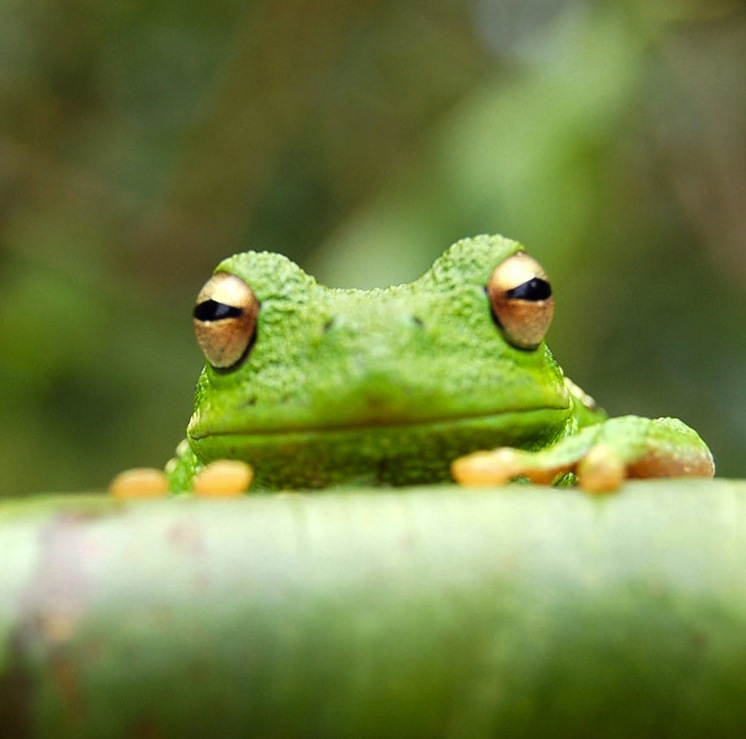
\includegraphics[scale=0.1]{frog}
\caption{Captions go beneath figures.}
\label{Frog}
\end{figure}

\begin{table}[H]
\centering
\caption{Captions go above tables.}
\begin{tabular}{| l | c | c |}
\hline
Parameter & Symbol & Value \\ \hline
Residence Time & $\theta$ & 90 s \\ \hline
Hydraulic Gradient & $G$ & 500 $\mathrm{s^{-1}}$ \\
\hline
\end{tabular}
\label{Table}
\end{table}

After describing a particular result, within a paragraph, go on to connect your work to fundamental physics/chemistry/statics/fluid mechanics, or whatever field is appropriate. Analyze your results and compare with theoretical expectations; or, if you have not yet done the experiments, describe your expectations based on established knowledge. Include implications of your results. How will your results influence the design of AguaClara plants? If possible provide clear recommendations for design changes that should be adopted. Show your experimental data in a professional way using the following guidelines:
\begin{itemize}
\item Why did you get those results/data?
\item Did these results line up with expectations?
\item What went wrong?
\item If the data do not support your hypothesis, is there another hypothesis that describes your new data?
\end{itemize}

\section*{Conclusions}
Explain what you have learned and how that influences your next steps. Why does what you discovered matter to AguaClara?
Make sure that you defend your conclusions. (this is conclusions, not opinions!)


\section*{Future Work}
Describe your plan of action for the next several weeks of research. Detail the next steps for this team. How can AguaClara use what you discovered for future projects? Your suggestions for challenges for future teams are most welcome. Should research in this area continue?

\bibliographystyle{apalike}
\bibliography{Bibliography}

\clearpage

\part*{Semester Schedule}

\subsection*{Task Map}
Task Maps should be created in Microsoft Word and then copy and pasted into the Detailed Task List in Overleaf. Save your word document on Google Drive so that you can make adjustments later in the semester.
To Create one, open Microsoft Word. Under Insert, go to Smart Art, click Hierarchy, then Horizontal Hierarchy.  Click the arrows on the left side of the box to open up a bulleted list of how your Map is organized. Make sure your map is as large as possible on the page (it may be necessary to increase the font size), then copy and paste it into the Google Doc.

\begin{figure}[H]
\centering
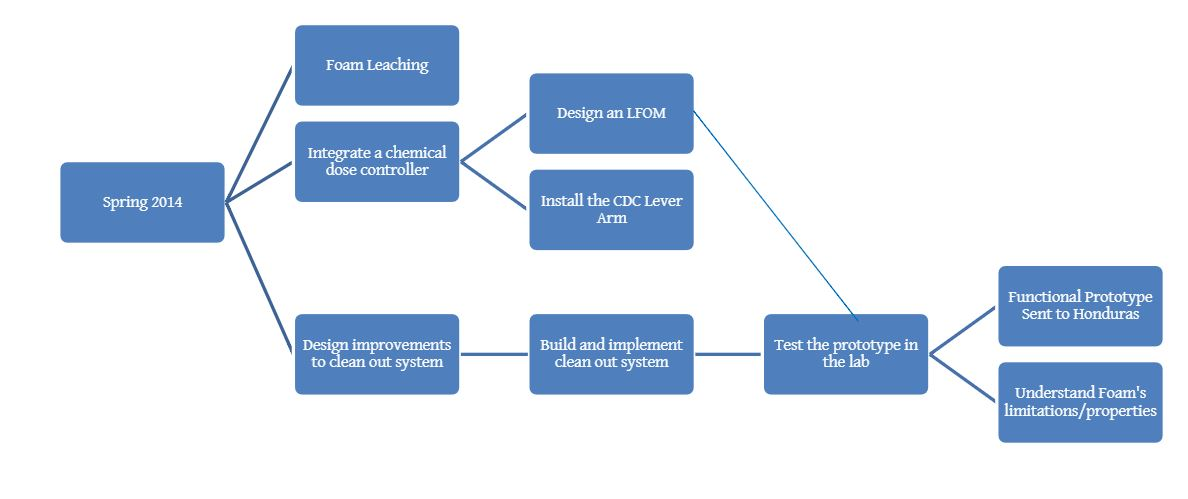
\includegraphics[scale=0.5]{ExampleTaskMap}
\caption{Example Task Map}
\label{ExampleTaskMap}
\end{figure}

\subsection*{Task List}
 You should keep and update your detailed task list from the first assignment in each of your reports. Denote completed tasks and modify your deadlines to reflect your most recently completed progress and any delays.

\begin{enumerate}
\item Task (date) - Individual responsible. Detailed explanation
\item \checkmark Task (date) - Individual responsible. This is an example of a completed task.

\end{enumerate}
\textbf{Report Proofreader: }Team member name

\clearpage

\part*{Manual}
The goal of this section is to provide all of the guidance that would be necessary for a future team to pick up your work where you left off. Please try to be thorough and put yourselves in the shoes of a newcomer to the project. Below are some recommended sections, but the manual will likely take a slightly different form for each team.

\section*{Experimental Methods}
\begin{enumerate}
\item Step 1.
\item Put tasks in a sequential order.
\item It is okay to have sub-lists.
	\begin{enumerate}
    \item Like this.
    \end{enumerate}
    \begin{itemize}
	\item Or like this.
	\end{itemize}
\item It is also okay to have multiple methods (e.g., in order to describe different steps in the experiment). For example:

\subsection*{Cleaning Procedure}
\begin{enumerate}
\item Step 1.
\end{enumerate}
\end{enumerate}

\section*{Experimental Checklist}
Another potential section could include a list of things that you need to check before running an experiment. Ideally, you would also have an Excel file for this, but you could give a more careful explanation of it here.

\section*{ProCoDA Method File}
Use this section to explain your method file (\texttt{.pcm}). This could be broken up into several components as shown below:

\subsection*{States}
Here, you should describe the function of each state in your method file, both in terms of its overall purpose and also in terms of the details that make it distinct from other states. For example:
\begin{itemize}
\item \underline{OFF} - Resting state of ProCoDA. All sensors, relays, and pumps are turned off.
\end{itemize}

\subsection*{Set Points}
Here, you should list the set points used in your method file and explain their use as well as how each was calculated.

\section*{Special Components}
If your subteam uses a particular part that is unique and you could foresee a future subteam needing to order it or learn more about it, please include basic information like the vendor where it was purchased, catalog/item number, and a link to any documentation. For example, here is a link to the \href{http://media.wattswater.com/OM-24034_MicroTOL_Series.pdf}{User's Manual} for the model of turbidimeter most commonly used in AguaClara research.
\end{document}
